\documentclass[book.tex]{subfiles}
\begin{document}
\section{Getting the Source Code}
The game engine source code was uploaded on id software's ftp\footnote{File Transfer Protocol.} server on July 21st, 1995.\\ 
\par
\begin{minipage}{\textwidth}
\lstinputlisting[]{code/ftp_url.txt}
\end{minipage}
\par
More than twenty two years later the archive is still located at the exact same URL, a remarkable fact given the ever changing nature of the web.\\

\section{First Contact}
Once downloaded and decompressed, the archive \codeword{woldsrc.zip} contains another self-extracting PKZIP archive. It was a convenience back in the day, but is not practical now and is easy to deflate.\\
\par
\begin{minipage}{\textwidth}
\lstinputlisting{code/unzip.txt}
\end{minipage}

\par
\cw{cloc.pl} is a tool which looks at every file in a folder and gathers statistics about source code. It helps for getting an idea of what to expect.\\
\par

\begin{minipage}{\textwidth}
\lstinputlisting[]{code/cloc.txt}
\end{minipage}

\par
 The code is 90\% in C with assembly\footnote{All the assembly in Wolf3D is done with TASM (a.k.a Turbo Assembler by Borland). It uses Intel notation where the destination is before the source: \cw{instr} \cw{dest} \cw{source}.} for bottleneck optimizations and low level I/O such as video or audio\footnote{id Software would not switch to C++ until Doom 3 around 2000.}. Lines of code (SLOC) is not a meaningful metric against a single codebase but excels when it comes to extracting proportions. Wolfenstein 3D with its 27,223 SLOC is very small compared to most software. \cw{curl} (a command-line tool to download url content) is 154,134 SLOC. Google's Chrome browser is 1,700,000 SLOC. Linux kernel is 15,000,000 SLOC.\\
\par
\begin{figure}[H]
\centering
  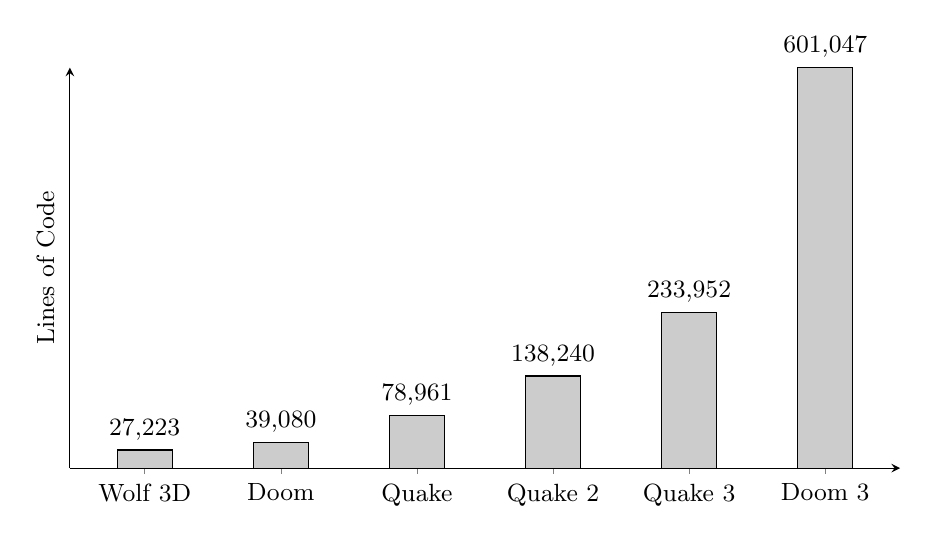
\begin{tikzpicture}[font=\small]
    \begin{axis}[
      width=\textwidth,
      height=0.55\textwidth,
      ybar=0.6\textwidth,
      bar width=20pt,
      ylabel={Lines of Code},
      ymin=0,
      ytick=\empty,
      xtick=data,
      axis x line=bottom,
      axis y line=left,
      enlarge x limits=0.11,
      symbolic x coords={Wolf 3D,Doom,Quake,Quake 2,Quake 3, Doom 3},
      xticklabel style={},
      yticklabel style={},
      nodes near coords={\pgfmathprintnumber[fixed,precision=0]\pgfplotspointmeta}
    ]
      \addplot[fill=black!20,draw=black] coordinates {
        (Wolf 3D,27223)
        (Doom,39080)
        (Quake,78961)
        (Quake 2, 138240)
        (Quake 3, 233952)
        (Doom 3, 601047)
      };
    \end{axis}
   \end{tikzpicture} 
   \caption{Lines of code from id Software game engines.}
 \end{figure}
 
\par

 \begin{fancyquotes}
   We didn't have spell checkers in our editors back then, and I always had poor spelling.  The word "collumn" appears in the source code dozens of times.  After I released the source code, one of the emails that stands out in memory read:
 \bigskip \\
It's "COLUMN", you dumb FUCK!\\
 \bigskip \\
\textbf{John Carmack - Programmer}
 \end{fancyquotes}
 
The archive contains more than just source code; it also features:
\begin{itemize}
\item \codeword{GOODSTUF.TXT:} Two emails from fans (an ex-POW and a Microsoft employee) demonstrating the success of the game.
\item \codeword{SIGNON.OBJ:} The startup screen showing the system characteristics (RAM, EMS, XMS, Joystick, SoundCards) was linked in the binary. This weird design choice is explained later.
\item \codeword{GAMEPAL.OBJ:} Game palette. Hardcoded and linked in the executable for the same reason as \cw{SIGNON.OBJ}.
\item \codeword{README:} How to build. You can also find a complete tutorial in "Let's compile like it's 1992" on \cw{fabiensanglard.net}.
\item Many files resulting from a previous compilation attempt.
\end{itemize}







\section{Big Picture}
The game engine is divided in three blocks:
\begin{itemize}
\item 2D menu engine which lets the user configure the game.
\item 3D game renderer where the user spends most of her time.
\item Sound system which runs concurrently with either the 2D or 3D renderer. 
\end{itemize}
The three systems communicate via shared memory. The renderer writes music and sound requests to the RAM (also making sure the assets are ready). These requests are read by the sound "loop". The sound system also writes to the RAM for the renderers since it is in charge of the heartbeat of the whole engine. The renderers update the world according to the wall-time tracked by \cw{TimeCount} variable.
\par
\begin{figure}[H]
\centering
 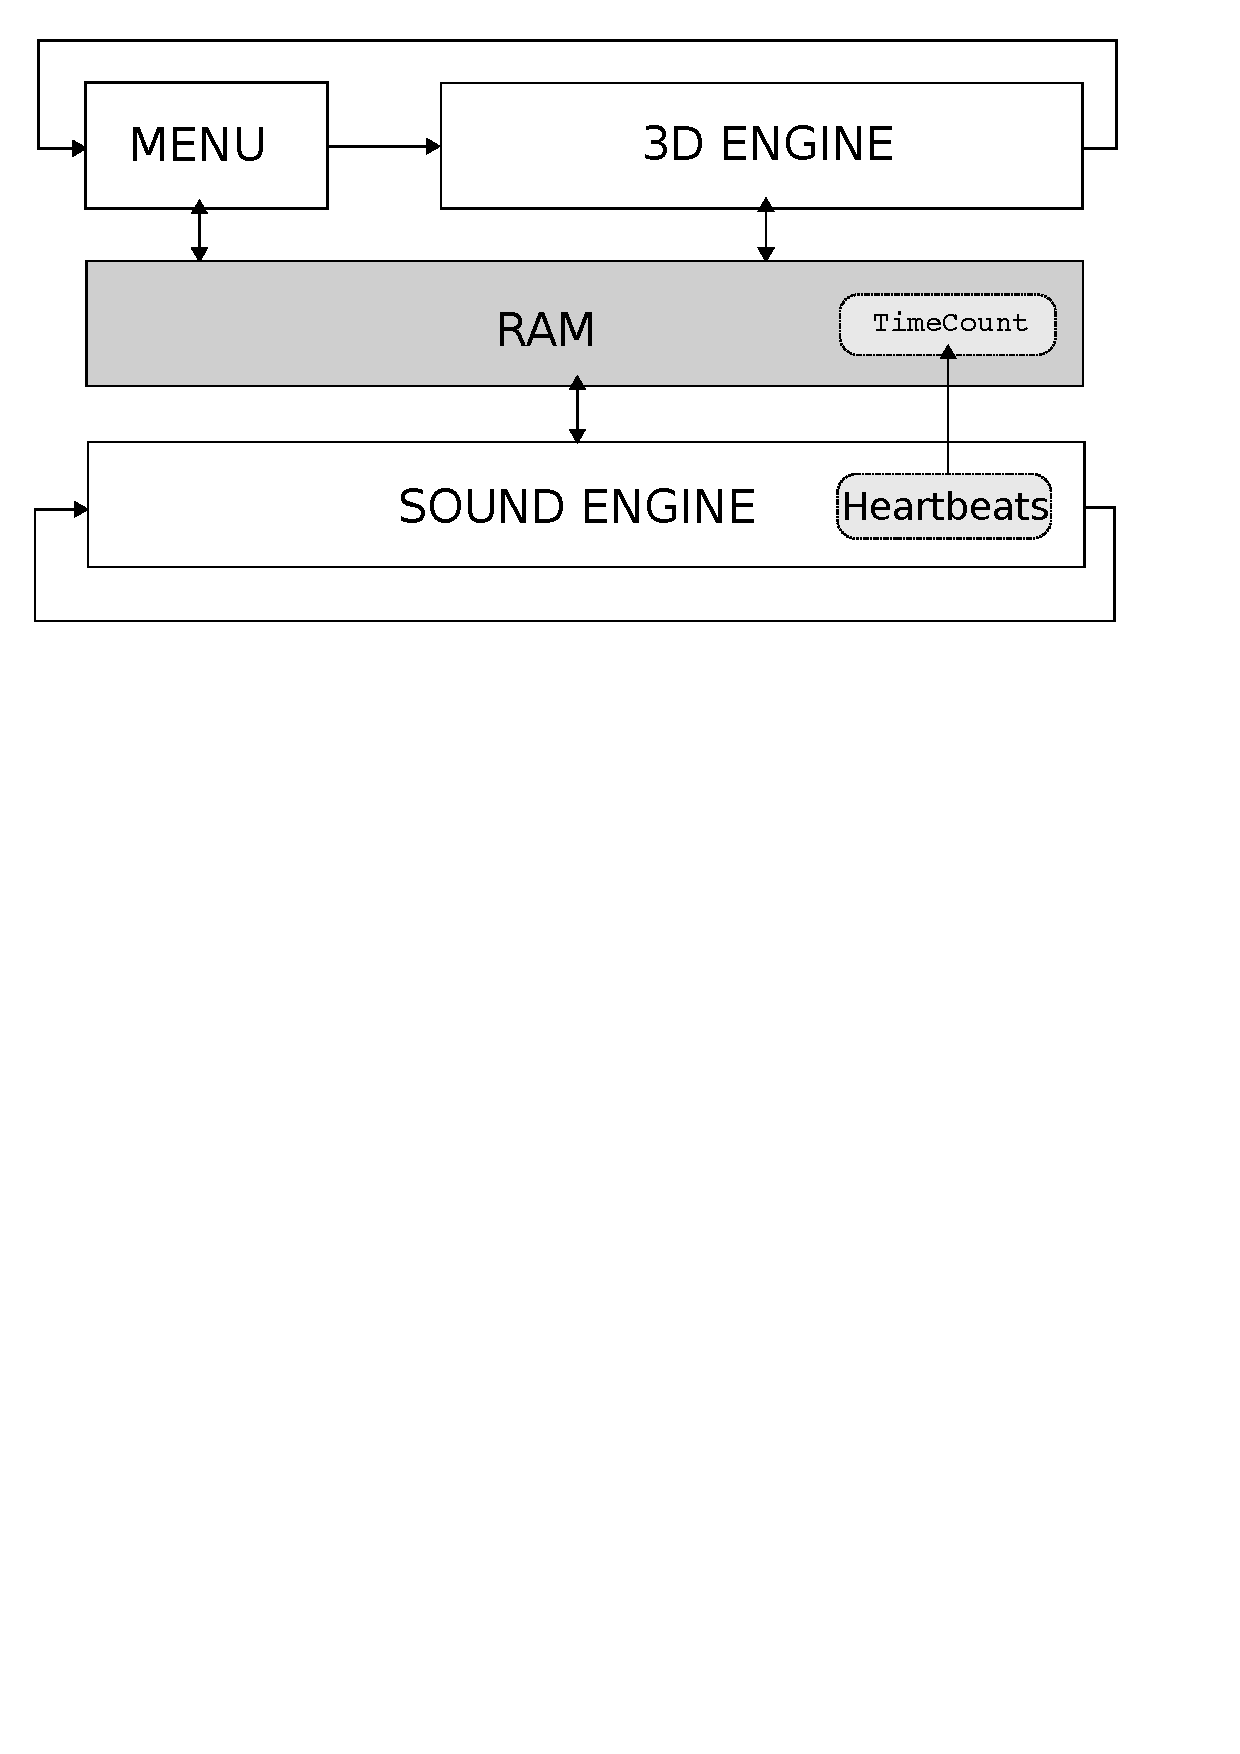
\includegraphics[width=\textwidth]{imgs/drawings/three_systems.pdf}
 \caption{Game engine three main systems.}
 \end{figure}
 \par

 









\subsection{Unrolled Loop}
With the big picture in mind, we can dive into the code and unroll the main loop starting in \cw{int main()}. The two renderers are regular loops but due to limitations explained later, the sound system is interrupt-driven and therefore out of \cw{main}. Because of real mode, C types don't mean what people would expect from a 32 bit architecture.
\begin{itemize}
\item \cw{int} and \cw{word} are 16 bit.
\item \cw{long} and \cw{dword} are 32 bit.
\end{itemize}
\par
The first thing the program does is check the assets available via \cw{CheckForEpisodes()}.\\
\par
\begin{minipage}{\textwidth}
\lstinputlisting[language=C]{code/unrolled_loop_main.c}
\end{minipage}
\par
Since the target machine ran in real mode, the code was compiled using 16 bit instructions only. For operations on \cw{long} (32 bit), Borland used its own math library. In \cw{Patch386} Wolfenstein 3D detects if the CPU is a 386 and patches its own code to replace Bordland's integral division with instructions using 32 bit registers \cw{eax} and \cw{edx}.\\
\par
\begin{minipage}{\textwidth}
\lstinputlisting[language={[x86masm]Assembler}]{code/integral_div.asm}
\end{minipage}
\par
In \cw{InitGame}, the engine starts up and brings up all the managers.\\
\par
\begin{minipage}{\textwidth}
\lstinputlisting[language=C]{code/unrolled_loop_init.c}
\end{minipage}
\par
Then comes the core loop, where the 2D renderer and 3D renderer are called forever.\\
\par
\begin{minipage}{\textwidth}
\lstinputlisting[language=C]{code/unrolled_loop_demoloop.c}
\end{minipage}
\par
\cw{PlayLoop} contains the 3D renderer. It is pretty standard with getting inputs, update world, and render world approach.\\
\par
\begin{minipage}{\textwidth}
\lstinputlisting[language=C]{code/unrolled_loop_playloop.c}
\end{minipage}
\par
The sound system is started via the Sound Manager in \cw{SDL\_SetTimerSpeed}. While there is a famous game development library called Simple DirectMedia Layer (SDL), the prefix \cw{SDL\_} has nothing to do with it. It stands for SounD Low level. (Simple DirectMedia Layer did not even exist in 1991).\\
\par
The reason for interrupts is extensively explained in Chapter \ref{audio_and_heartbeat} "\nameref{audio_and_heartbeat}". In short, with an OS supporting neither process nor thread, it was the only way to have something execute concurrently with the rest of the engine.\\
\par
An ISR\footnote{Interrupt Service Routine.} is installed in the Interrupt Vector Table to respond to interrupts triggered by the engine. Note how the ISR can be called at frequencies of 140Hz, 700Hz, or even 7000Hz depending on the needs of the sound system.\\
\par
\begin{minipage}{\textwidth}
\lstinputlisting[language=C]{code/soundsystem_interrupt.c}
\end{minipage}
\par
















\section{Architecture}

The source code is structured in two layers. WL\_* files are high-level layers relying on low-level ID\_* sub-systems called Managers interacting with the hardware.\\
\par
\begin{figure}[H]
\centering
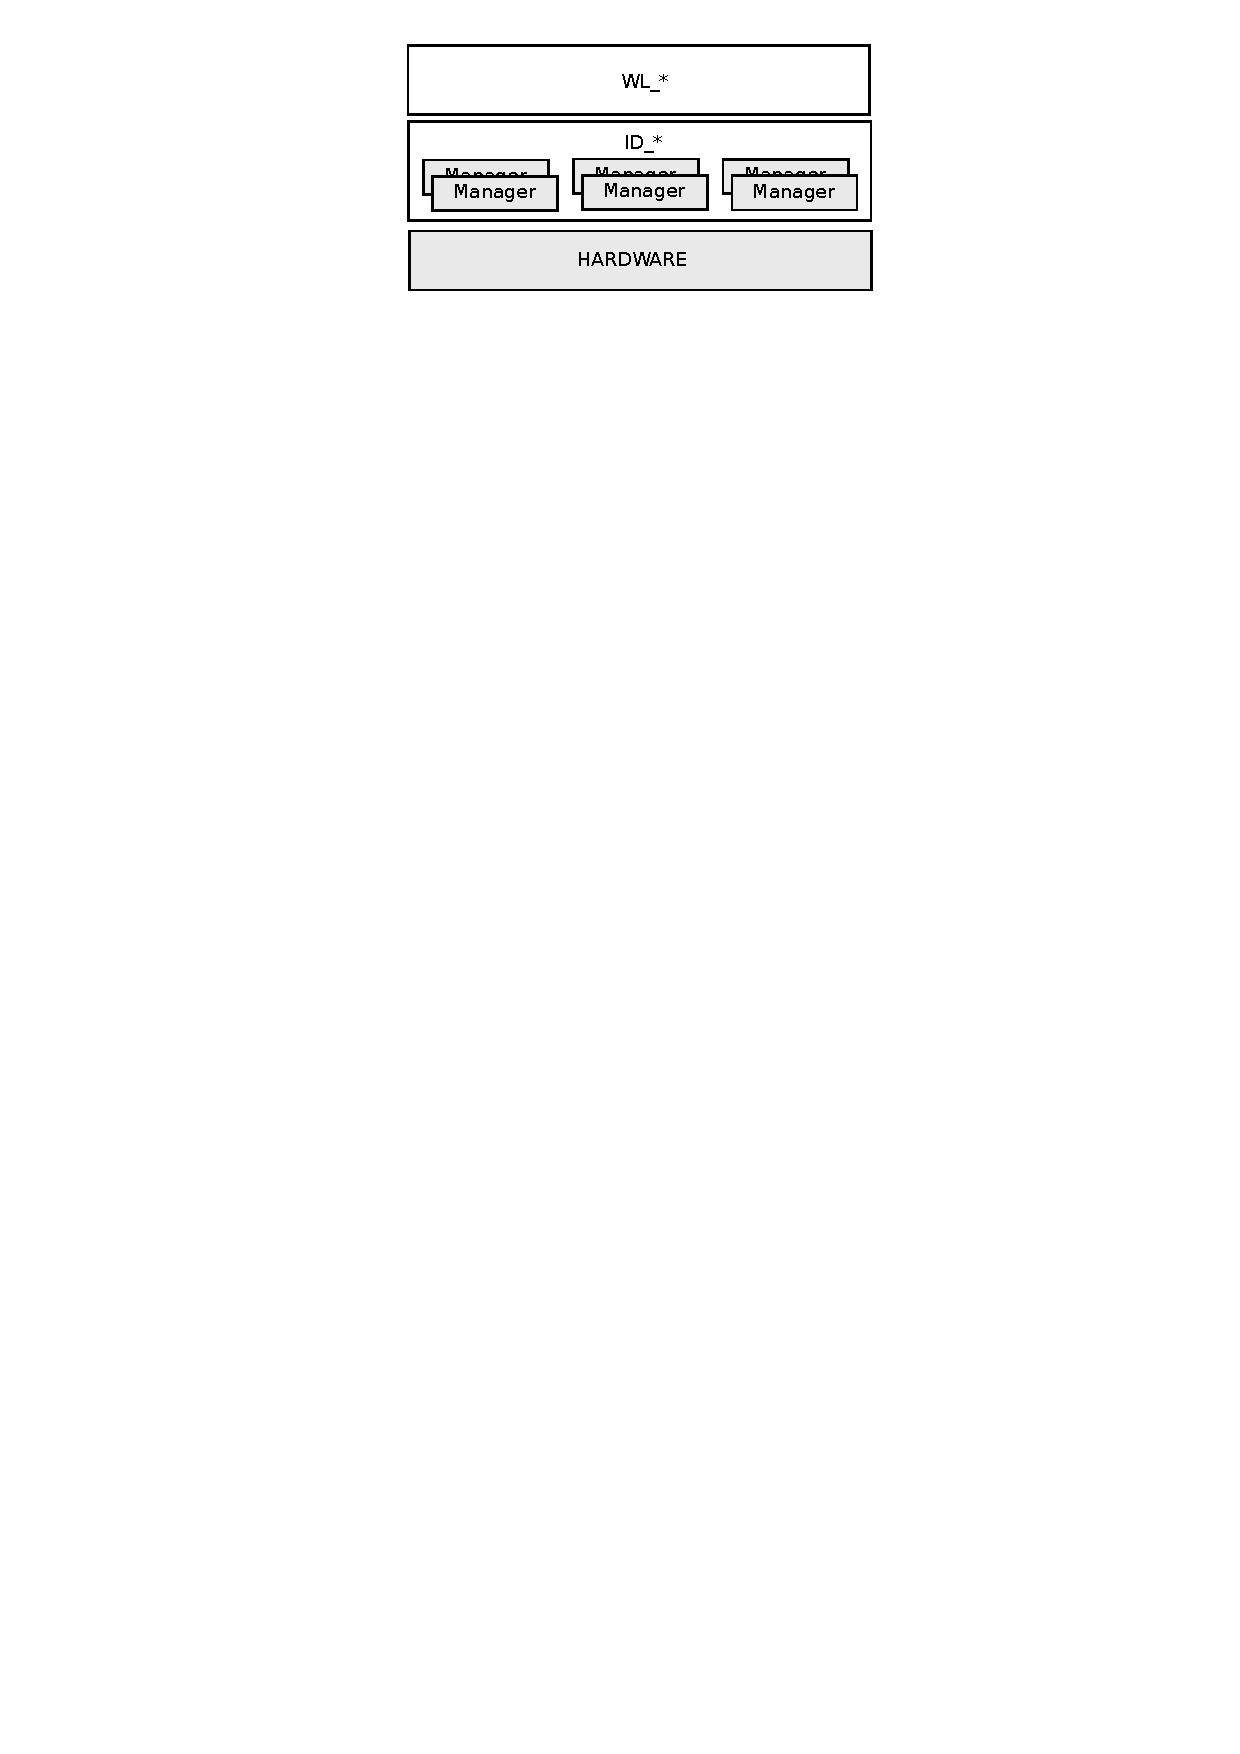
\includegraphics[width=\textwidth]{imgs/drawings/layers.pdf} 
\caption{Wolfenstein 3D source code layers.}
 \end{figure}
 \par
There are seven managers in total:\\

\begin{itemize}
	\item Memory
	\item Page
	\item Video
	\item Cache
	\item Sound
	\item User
	\item Input
\end{itemize}
\par
The WL\_ stuff was written specifically for Wolf3D while the ID\_ managers were reused from previous games (Hovertank 3D and Catacomb 3D) and improved for the needs of the new engine.

\begin{figure}[H]
\centering
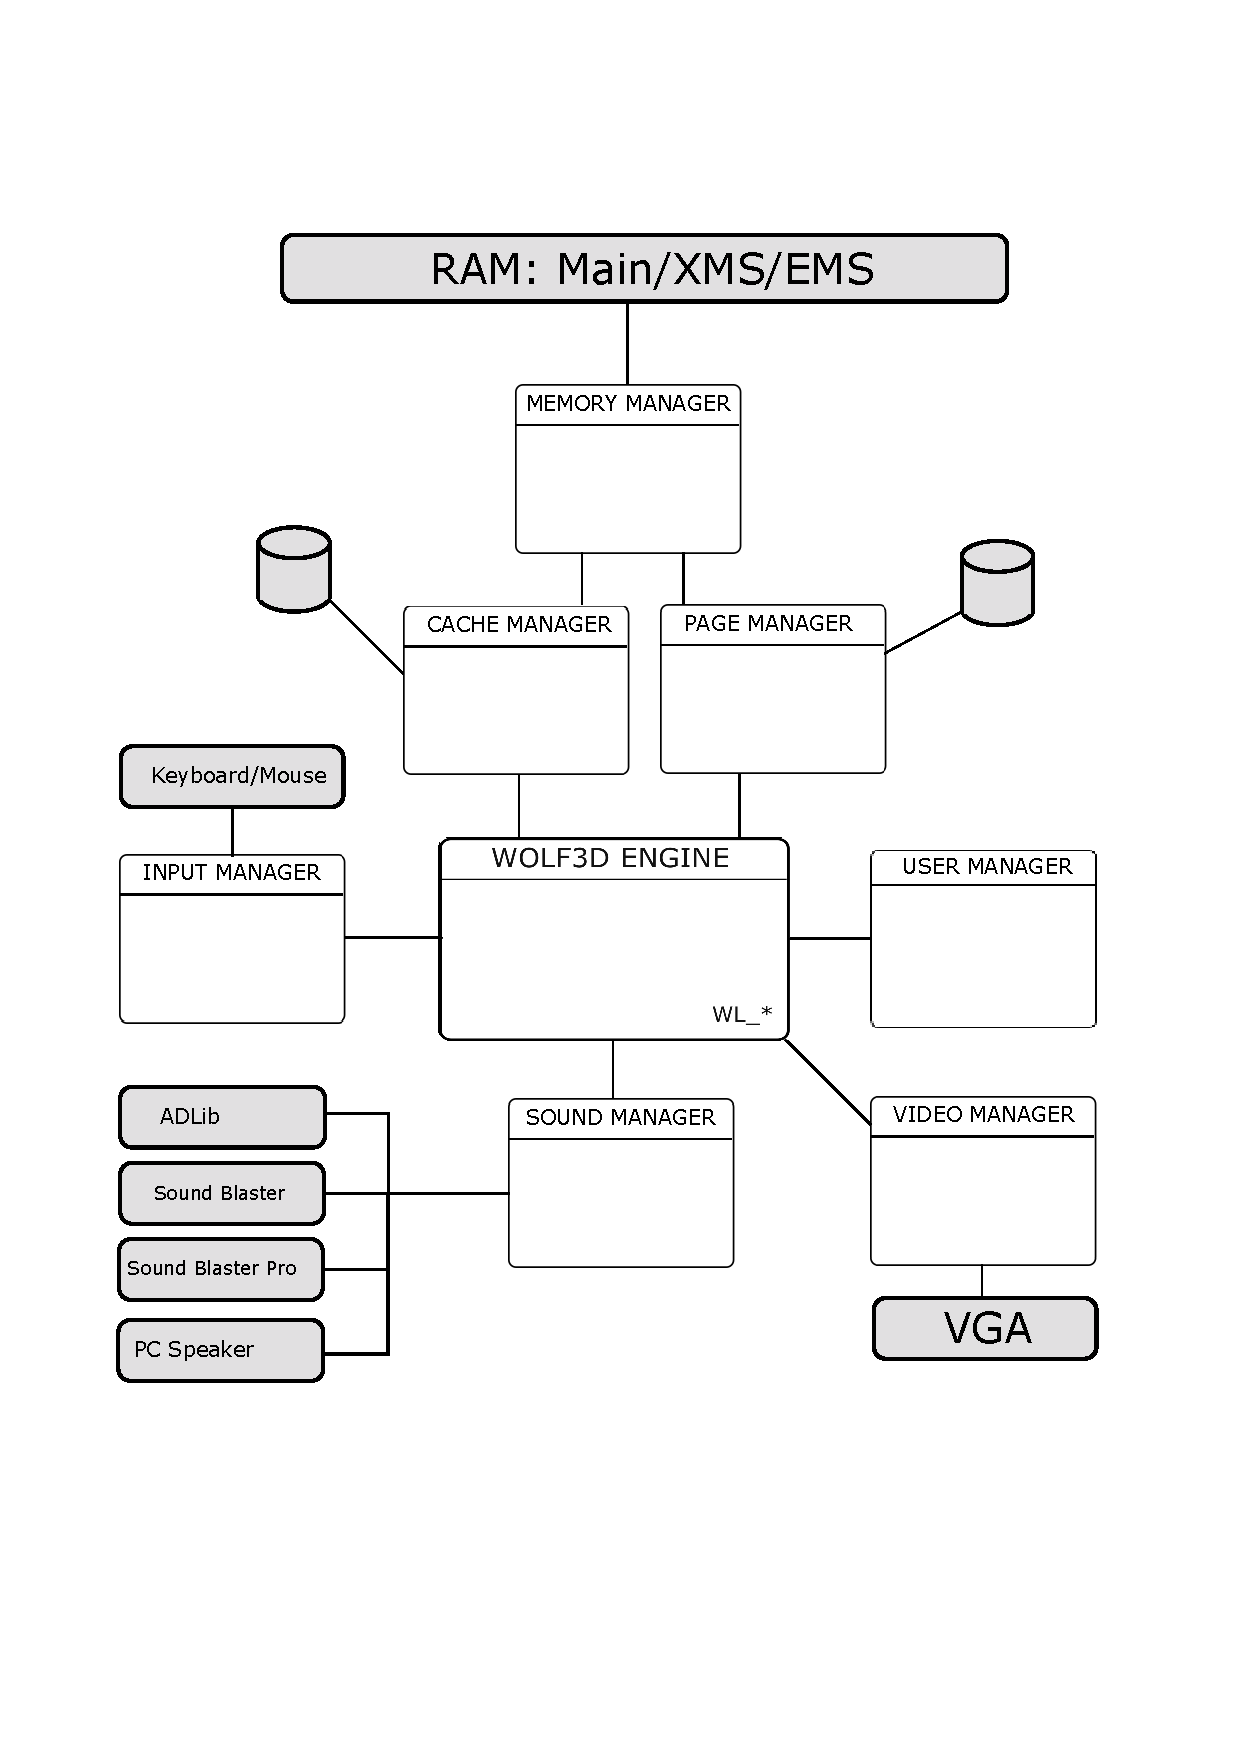
\includegraphics[width=\textwidth]{imgs/drawings/architecture.pdf}
\caption{Architecture with engine and sub-systems (in white) connected to I/O (in gray).}
\label{fig:architecture}
\end{figure}
Next to the hard drives (HDD) you can see the assets packed as described in Chapter \ref{chapter_team} Team.










\subsection{Memory Manager (MM)}
The engine does not rely on \cw{malloc} to manage conventional memory, as this can lead to fragmented memory and no way to compact free space. It has its own memory manager made of a linked list of "blocks" keeping track of the RAM. A block points to a starting point in RAM and has a size.\\
 \par
\lstinputlisting[language=C]{code/mm_block.c}
 \par
A block can be marked with attributes:
\begin{itemize}
\item \cw{LOCKBIT} : This block of RAM cannot be moved during compaction.
\item \cw{PURGEBITS} : Four levels available, 0= unpurgable, 1= purgable, 2= not used, 3= purge first.
\end{itemize}

The memory manager starts by allocating all available RAM via \cw{malloc}/\cw{farmalloc} and creates a \cw{LOCKED} block of size 1KiB at the end. The linked list uses two pointers: \cw{HEAD} and \cw{ROVER} which point to the second to last block.
 \par
\begin{figure}[H]
\centering
 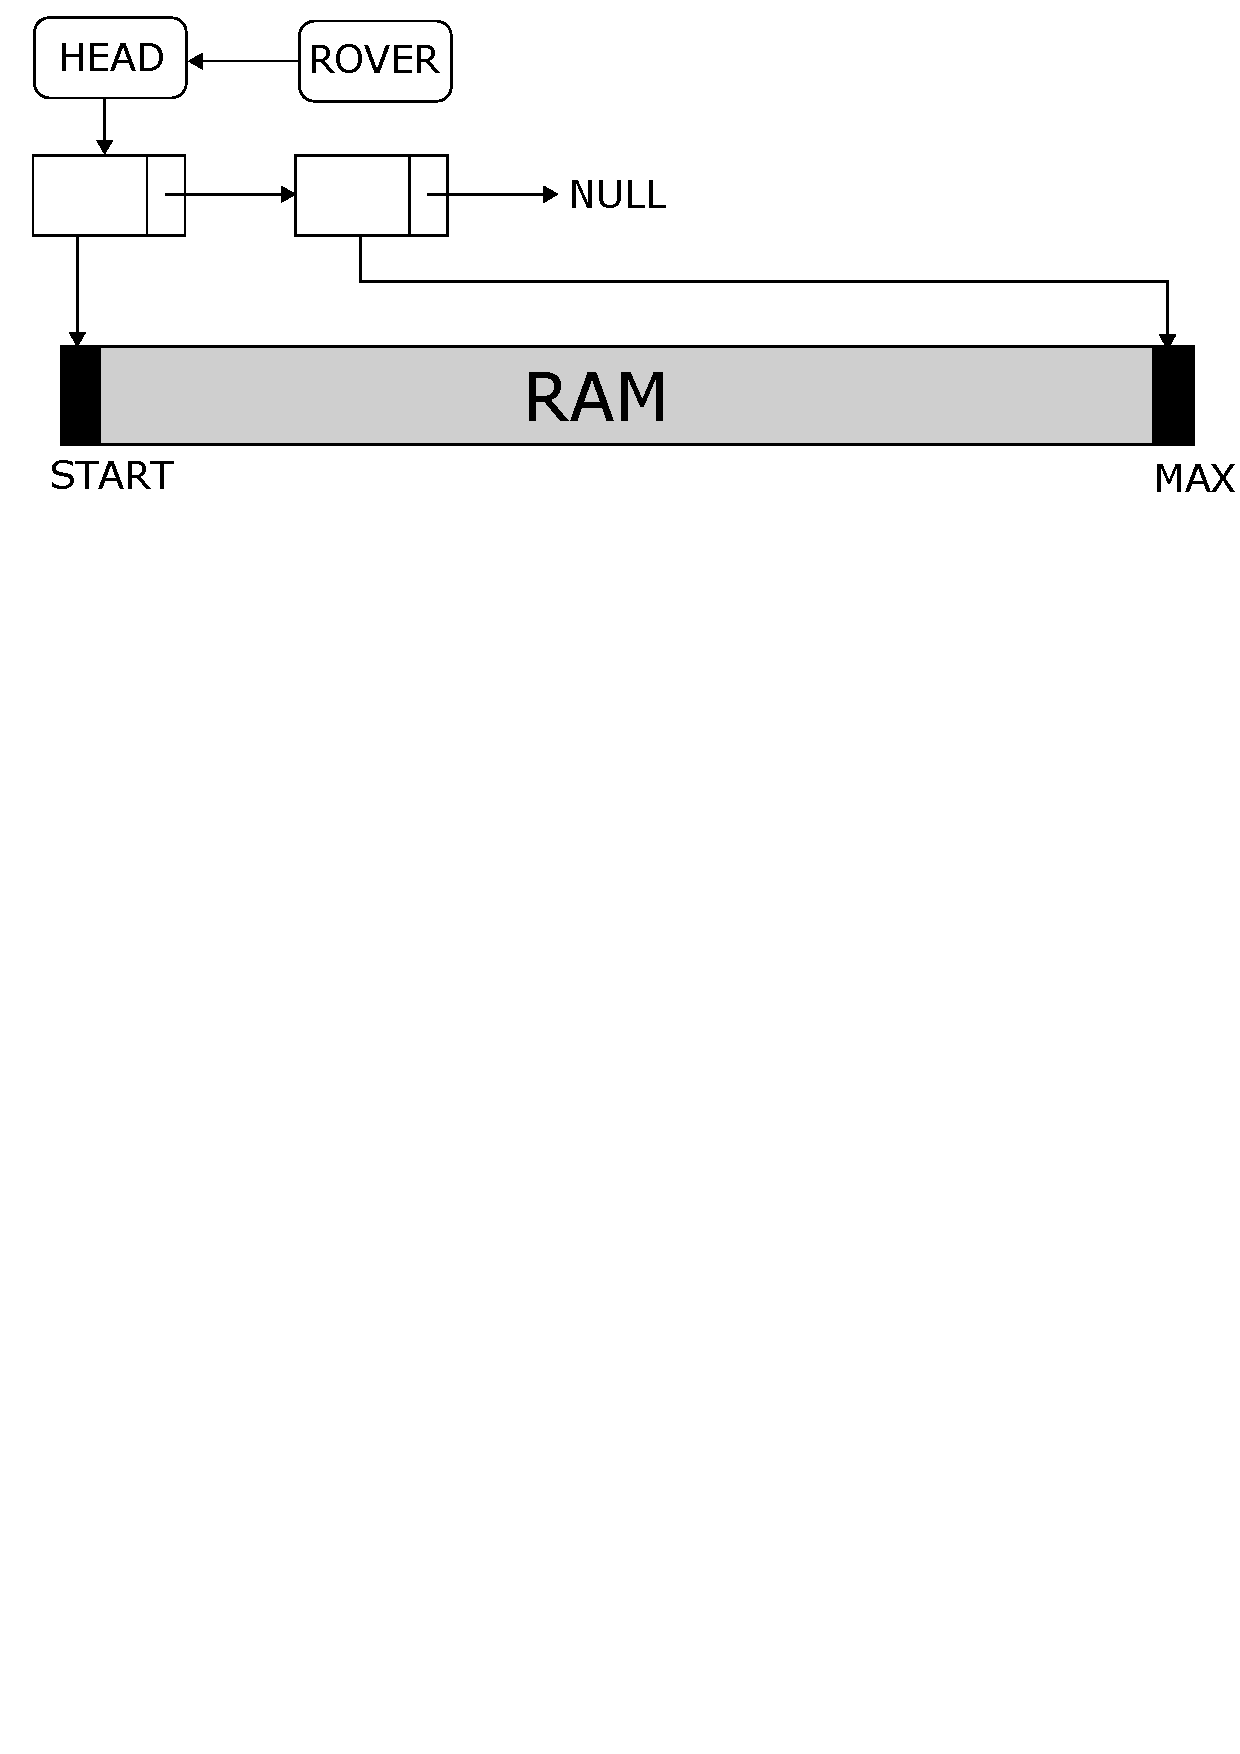
\includegraphics[width=\textwidth]{imgs/drawings/mm_start.pdf}
 \caption{Initial memory manager state.}
 \end{figure}
 \par
 The engine interacts with the Memory Manager by requesting RAM (\cw{MM\_GetPtr}) and freeing RAM (\cw{MM\_FreePtr}). To allocate memory, the manager searches for "holes" between blocks. This can take up to three passes of increasing complexity:
\begin{enumerate}
\item After rover.
\item After head.
\item Compacting and then after rover.
\end{enumerate}
\par
  The easiest case is when there is enough space after the rover. A new node is simply added to the linked list and the rover moves forward. In the next drawing, three allocation requests have succeeded: \cw{A}, \cw{B} and \cw{C}.\\
  \par
\begin{figure}[H]
\centering
 \includegraphics[width=\textwidth]{imgs/drawings/mm_after_rover.pdf}
 \caption{MM internal state after three pass 1 allocations.}
 \end{figure}
 \par
Eventually the free RAM will be exhausted and the first pass will fail.
  \par
\begin{figure}[H]
\centering
 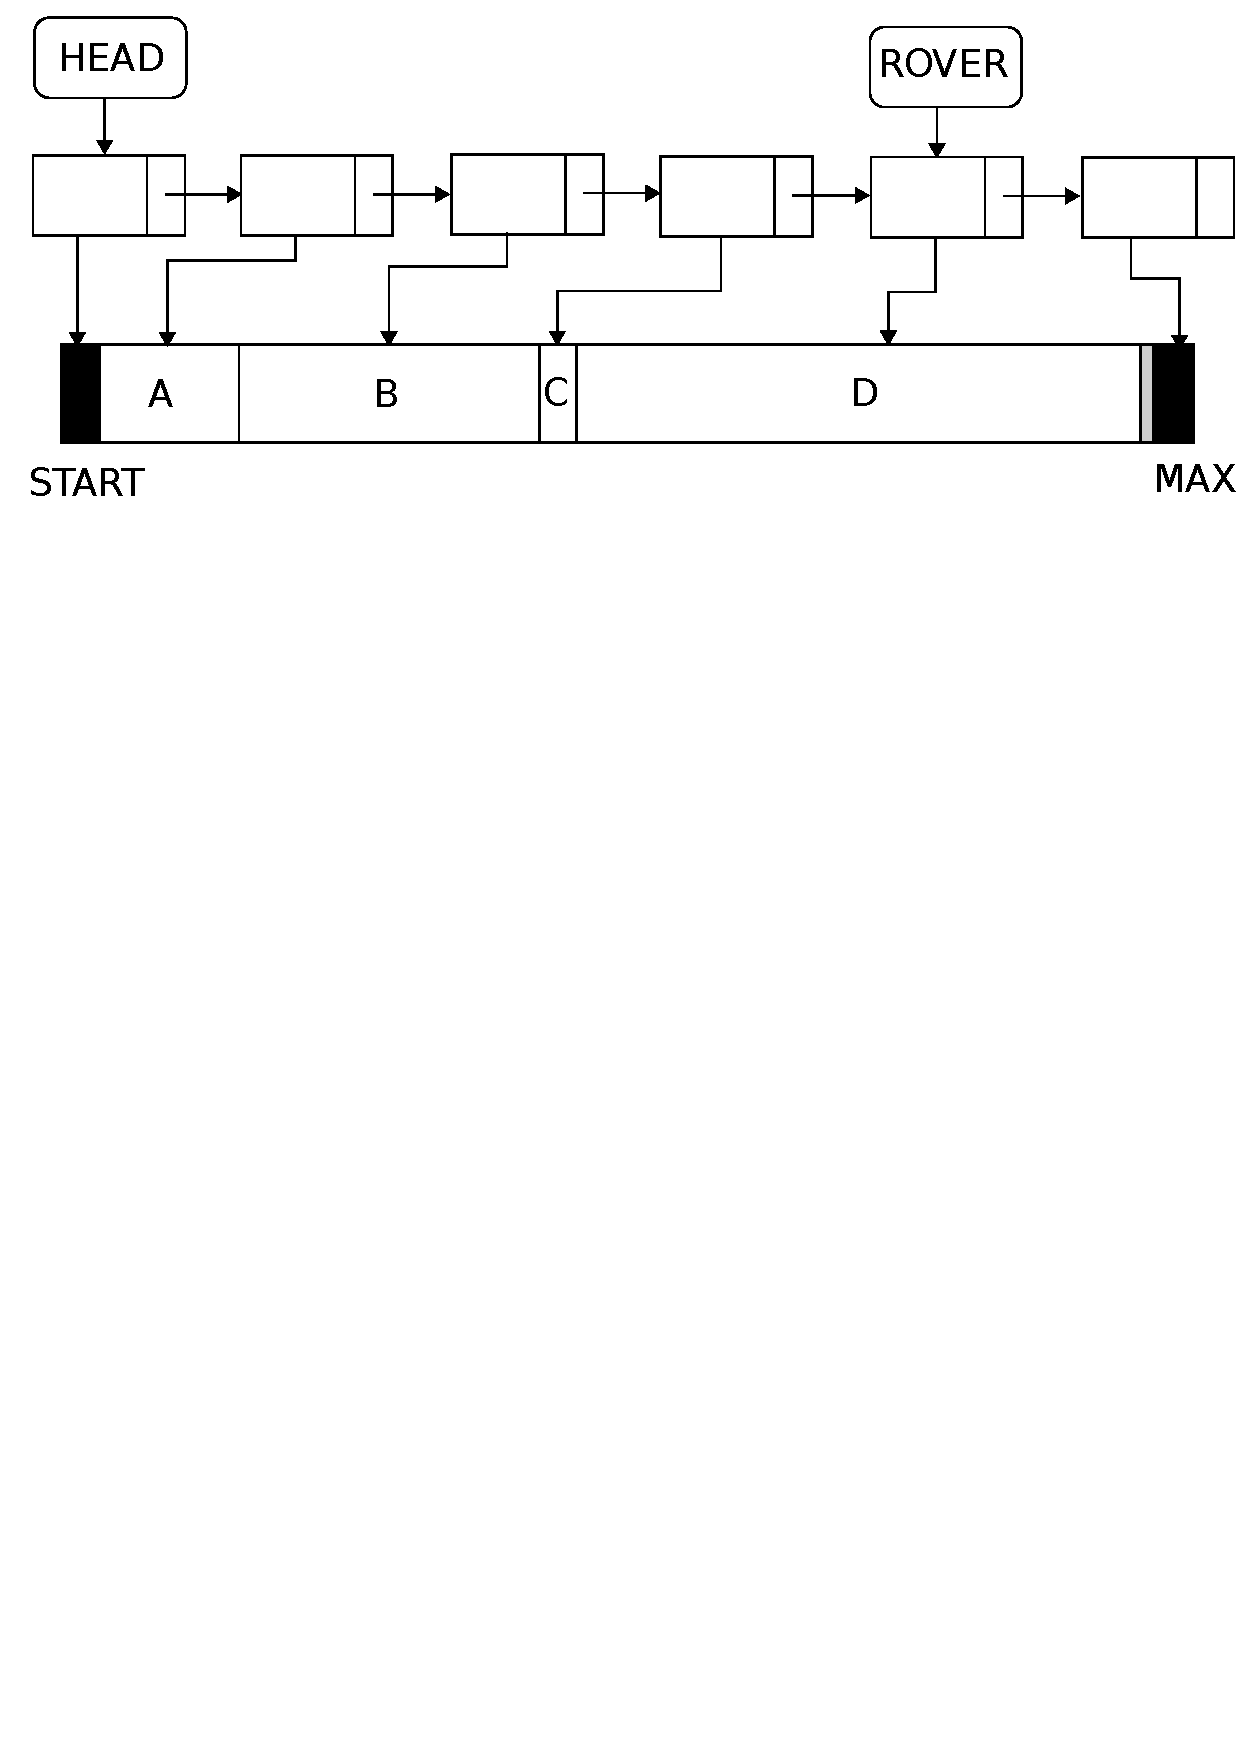
\includegraphics[width=\textwidth]{imgs/drawings/mm_before_rover.pdf}
 \caption{Pass 1 failure: Not enough RAM after the ROVER.}
 \end{figure}
 \par
 If the first pass fails, the second pass looks for a "hole" between the head and the rover. This pass will also purge unused blocks. If for example block B was marked as \cw{PURGEABLE}, it will be deleted and replaced with the new block E. At this point fragmentation starts to appear (like if \cw{malloc} was used).\\
 \begin{figure}[H]
\centering
 \includegraphics[width=\textwidth]{imgs/drawings/mm_after_head.pdf}
 \caption{\cw{B} was purged. \cw{E} was allocated in pass 2.}
 \end{figure}
 \par
 If the first and second pass fail, there is no continuous block of memory large enough to satisfy the request. The manager will then iterate through the entire linked list and do two things: delete blocks marked as purgeable, and compact the RAM by moving blocks.
  \par
\begin{figure}[H]
\centering
 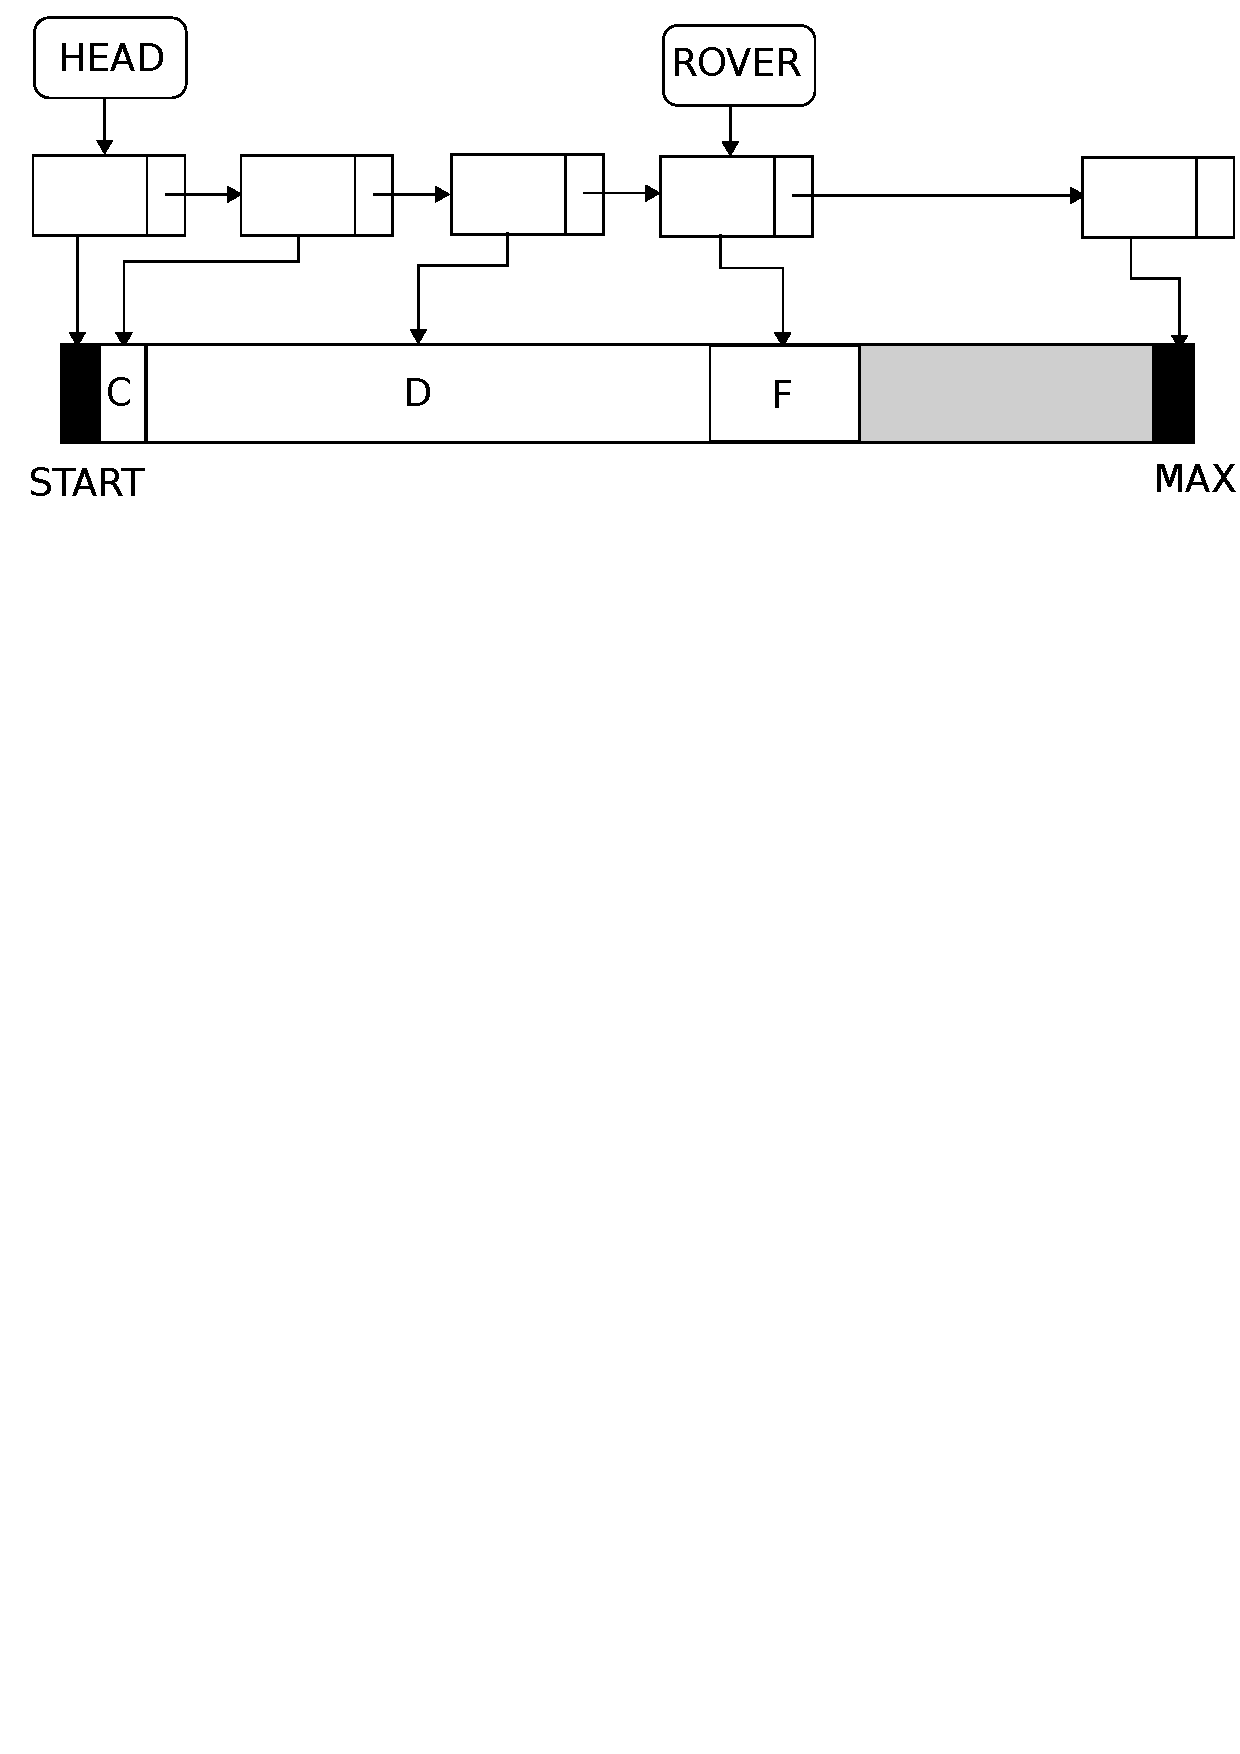
\includegraphics[width=\textwidth]{imgs/drawings/mm_compact.pdf}
  \caption{\cw{A} and \cw{E} were purged. \cw{C} and \cw{D} compacted. \cw{F} allocated in pass3.}
 \end{figure}
 \par
But if memory is moved around, how do previous allocations still point to what they did before the compaction phase? Notice that a \cw{mmblockstruct} has a \cw{useptr} pointer which points to the owner of a block.  When memory is moved, the owner of the block is also updated.\\
\par
As some blocks are marked as \cw{LOCKED}, compacting can be disturbed. Upon encountering a locked block, compacting stops and the next block will be moved immediately after the locked block, even if there was space available between the last block and the locked block.\\
   \par
\begin{figure}[H]
\centering
 \includegraphics[width=\textwidth]{imgs/drawings/mm_bad_compact.pdf}
 \caption{\cw{E} is locked and cannot be compacted.}
 \end{figure}
 \par
  In the above drawing, C was moved after E, even though it could have been moved before. Avoiding this waste would have made the memory manager more complicated, so the waste was deemed acceptable. Often in designing a component you have to be practical and establish a certain trade off between accuracy and complexity.\\
  \par



\begin{fancyquotes}
A dedicated memory manager was probably justified for Wolf, but they are a huge source of bugs, and I urge people not to do it!\\
\par
\textbf{John Carmack - Programmer}
 \end{fancyquotes}






\subsection{Page Manager (PM)}
The Page Manager is dedicated to the 3D engine. Its task is to make sure assets such as wall textures, sprites, and sound effects stored on HDD are available in RAM for the CPU to use. Jason Blochowiak seems to have been the main author and his previous experience with Unix clearly influenced the design of this component. It is built around the concept of paging and swapping. \\
\par
Instead of using a memory address to identify a page like Unix, an asset ID is used. These IDs are generated by IGRAB-ED. Each asset consumes a full "page". Like Unix, all pages have the same size, 4KiB. When the engine needs a resource, it requests a page with the resource ID from the Page Manager. All types of RAM (Conventional, EMS, and XMS) are leveraged but there is a hierarchy.\\
\par
Originally all assets for 3D sequences are on HDD in file \cw{VSWAP.WL1}. When a request for an asset is received, the L1 cache (comprised of Conventional and EMS RAM) is looked up first \circled{1}. In case of a miss, the L2 cache is consulted \circled{2}. If the page is found there, it is transferred to L1. If the page is still not found in L2, it is loaded from the HDD directly to L1 \circled{3}. L2 is only written to when a page is evicted from L1. Every time a page is accessed, it is also tagged with the current frame number. This tag is used to enforce the eviction policy.
 \par
\begin{figure}[H]
\centering
 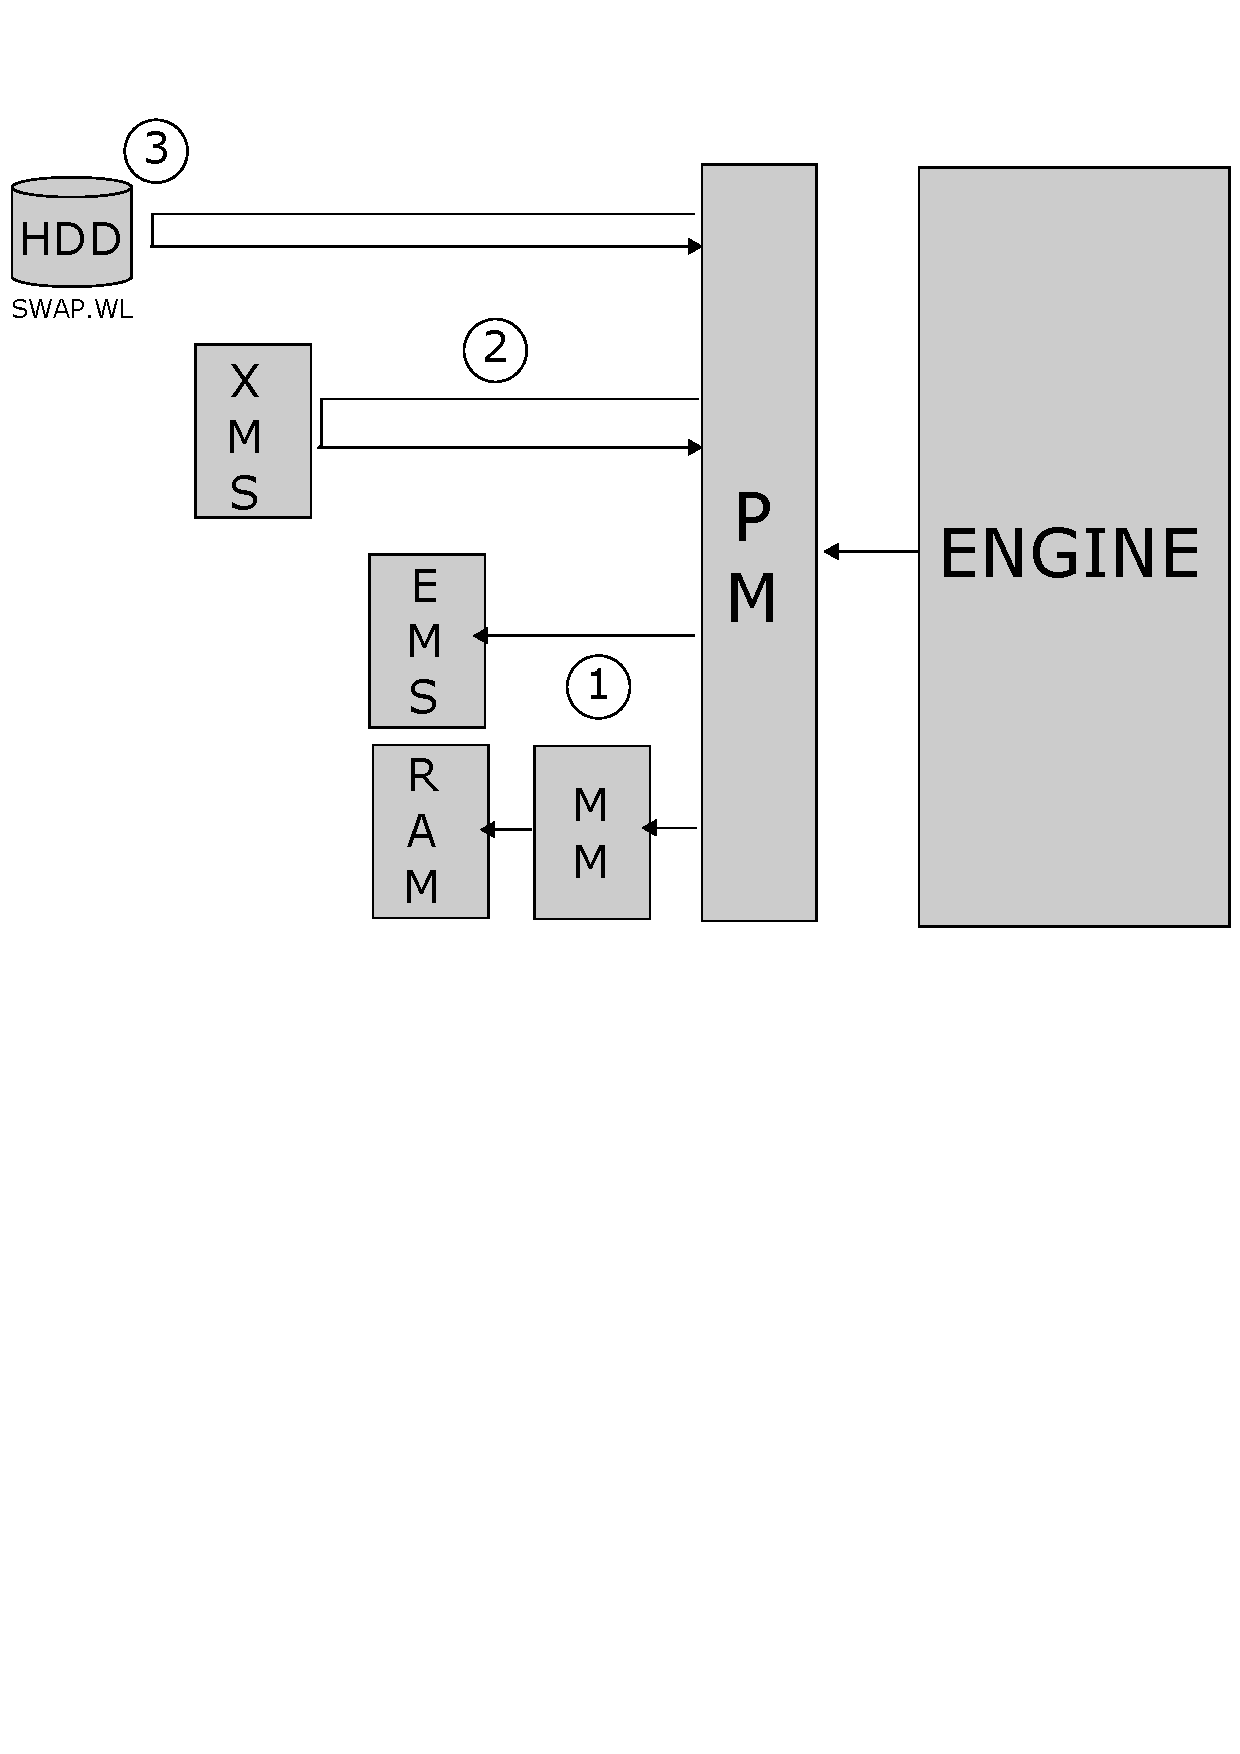
\includegraphics[width=\textwidth]{imgs/drawings/page_manager_architecture.pdf}
 \end{figure}
 \par
 The architecture of the Page Manager is interesting since it treats XMS as a last resort L2 cache level while EMS RAM is used like conventional memory. This is because EMS driven RAM is several time faster than XMS driven RAM and almost as fast as conventional memory. This topic is detailed in Annexe \ref{ems_vs_xms} on page \pageref{ems_vs_xms}\\
 \par
In order to minimize the cost of page misses, the engine preloads the page cache before a level start. The user experiences this as the "Get Psyched" screen:
 \par
\begin{figure}[H]
\centering
 \fullimage{get_psyched.png}
 \caption{The "thermometer" showing the Page Manager precaching process.}
 \end{figure}
 \par
The precaching mechanism is not particularly clever: it loads as many pages from the swap file as possible. It doesn't try to look at what is actually used in the level but instead loads assets in the order they are stored in \cw{VSWAP} file on the HDD. On a machine with low memory (less than 1MB), the eviction policy (LRU) stabilizes the cache after a few minutes in a level.\\
\par
This design has a small yet annoying flaw. On a low memory machine, a cache miss will occur when the player opens the last door of a level and is about to find herself confronted with the heavy-power final boss. This enemy has never been seen before, and therefore is not in the cache of the Page Manager. This incurs the worst possible case of cache miss: a long access to the hard-drive is required, leading to lag and often resulting in an undeserved (and humiliating) death.\\
\par
The size of the swap file varies depending on the version of the game being played: \cw{VSWAP.WL1} (shareware) is 742KiB while \cw{VSWAP.WL6} (full version) is 1,500KiB. In both cases a machine with 2MiB of RAM on top of the factory issued 1MiB is enough to have all assets loaded during precaching.\\
\par
\bu{Thrashing:} When the system has to evict pages but ends up reloading the same resource during the same frame, "thrashing" occurs. The HDD is put to heavy use, and framerate drops. Trashing can happen if too many different resources are visible on the screen. In order to help designers balance their creativity with the need for a decent framerate, the engine detects trashing and flashes the screen border red when running in dev-mode.\\
\par
\bu{Sounds are special:} Because sound cards are fed via a system of interrupts, the sound manager cannot recover from a page miss. Therefore, all sound resources are loaded first (they are located at the start of \cw{SWAP.WL1}) and only in conventional memory.











\subsection{Video Manager (VL \& VH)}
The video manager features two parts:
\begin{itemize}
\item A low level dedicated to hardware VGA register manipulation.
\item A high level dedicated to 2D menu drawings.
\end{itemize}
\par






\subsection{Cache Manager (CA)}
The cache manager is a small but critical component. It loads and decompresses maps, 2D graphics, and audio resources stored on the filesystem and makes them available in RAM. Assets of each kind are stored in two files. A header file contains the offset to allow translation from asset ID to byte offset in the data file.\\
 \par
\begin{figure}[H]
\centering
 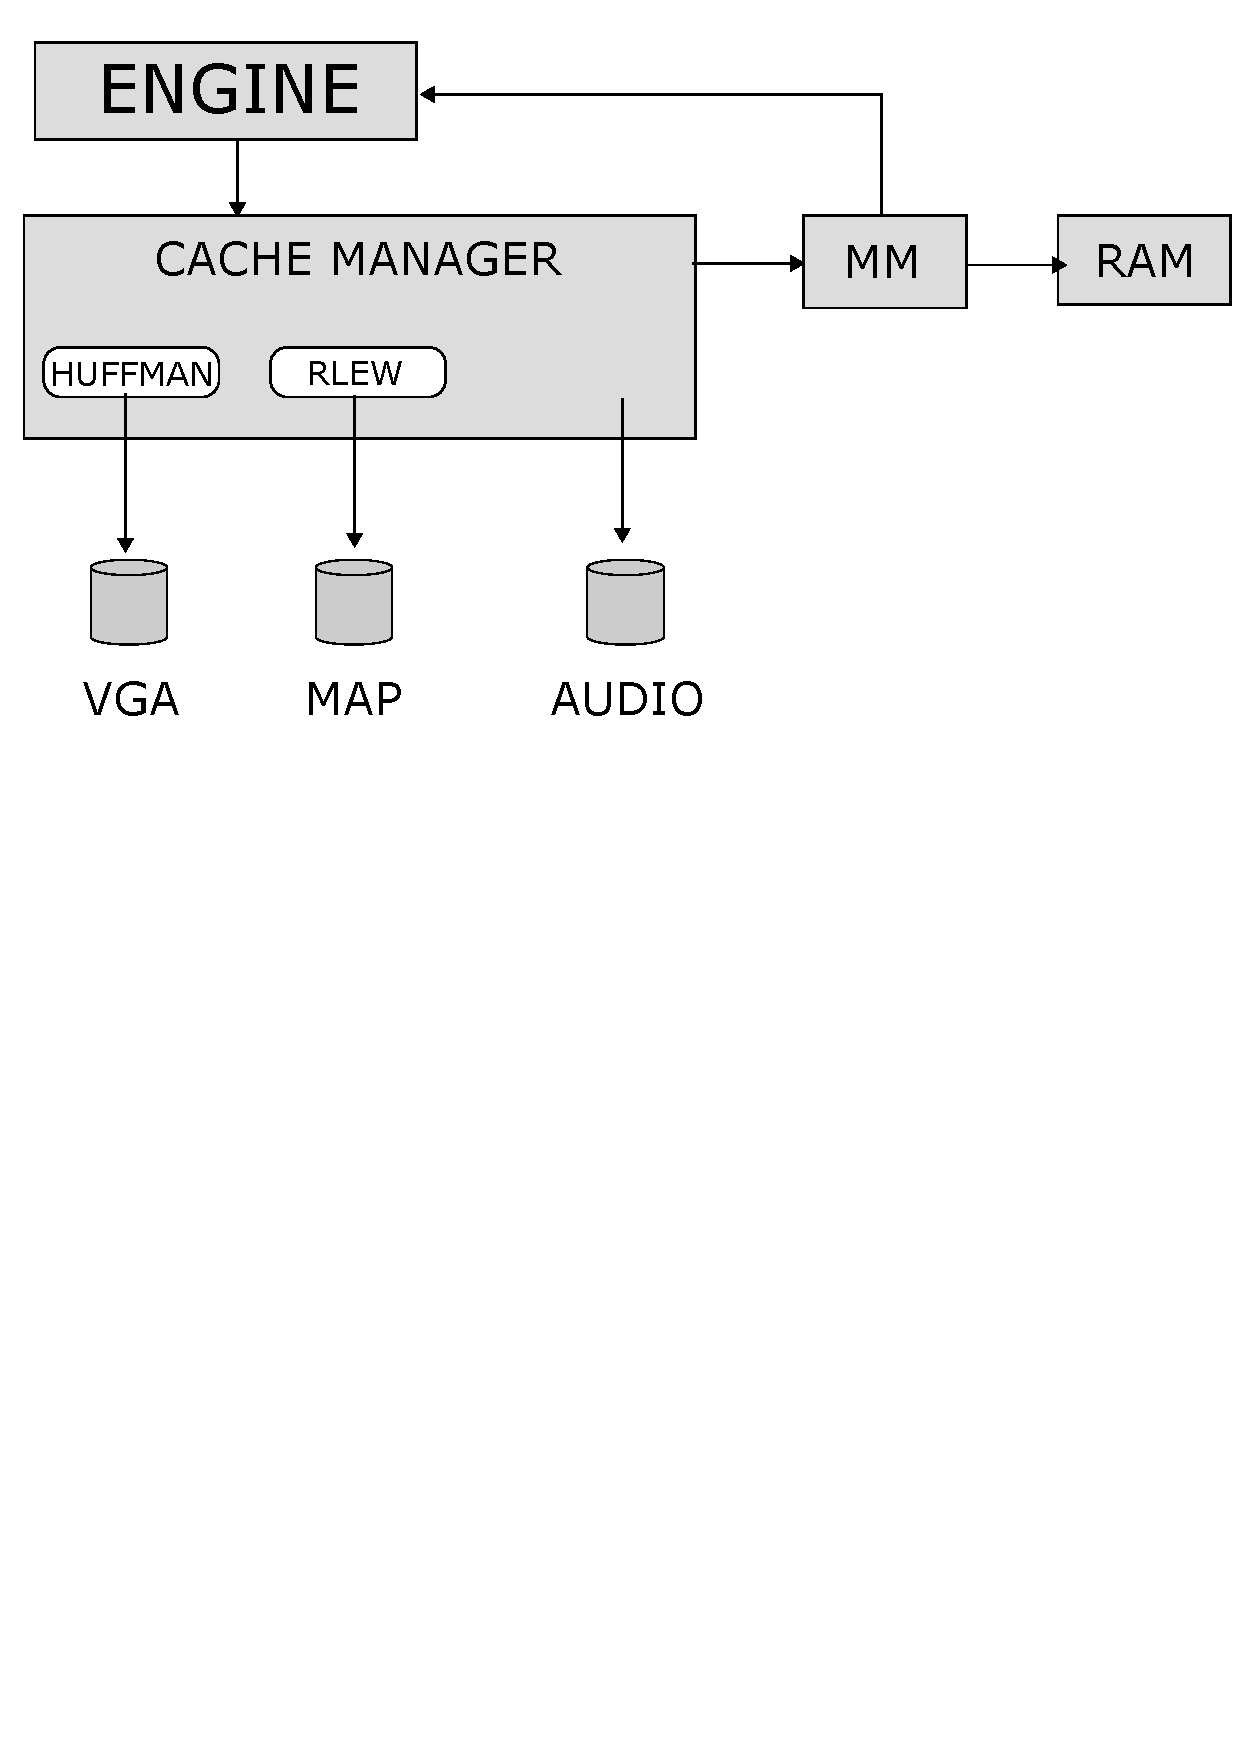
\includegraphics[width=\textwidth]{imgs/drawings/cache_manager_architecture.pdf}
 \end{figure}
 \par
\bu{Note:} All resources are compressed. In the case of maps and audio, compression is hard-coded in the engine. For graphics, however, a third file (\cw{DICT}) contains the compression dictionary to decompress each asset. The Cache Manager handles decompression transparently.\\
\par
\bu{Trivia :} Is there a typo in the filename \cw{AUDIOHED.WL} ? The correct spelling would be \texttt{\justify AUDIOHEAD.WL1}. Where is the \cw{A}? This is in fact a limitation of the operating system. DOS only allows 8.3 filename (at most eight characters followed by a dot, then at most three characters for the extension).








\subsection{User Manager (US)}
\begin{minipage}{0.7\textwidth}
The User Manager is largely based on the Catacomb 3D code and was written by Jason Blochowiak. The copy/paste is very visible since 90\% of the functions declared in the header (ID\_US.H) are not actually implemented in \cw{ID\_US.C}. 
It is a poorly named manager as it mostly takes care of text layout. When a \cw{WL\_*} high level routine needs to draw a string, it is passed to \cw{US\_Print} which does all measurement (e.g. Draw string centered)
and then passes this information to the Video Manager (\cw{VW\_DrawPropString}), which takes care of rendition.
\end{minipage}
\begin{minipage}{0.3\textwidth}
\begin{flushright}
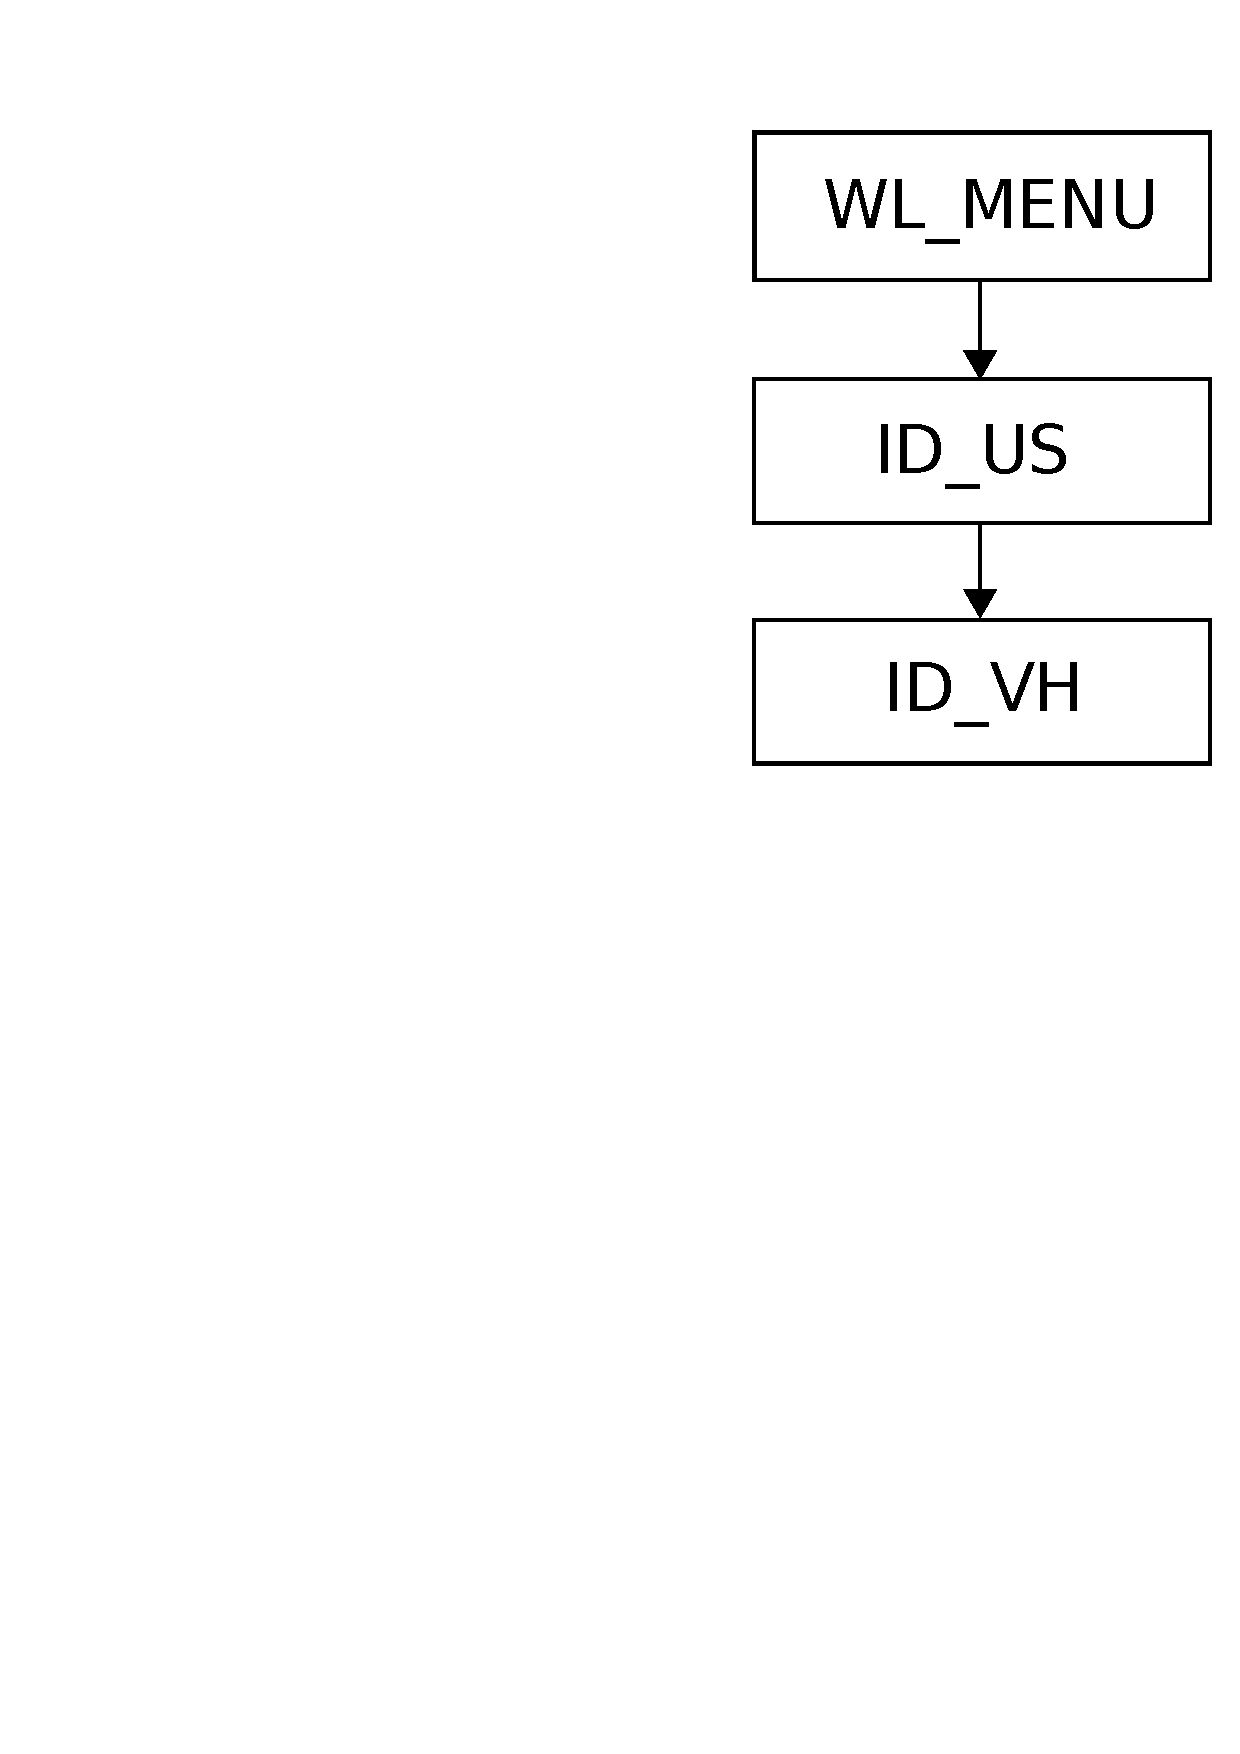
\includegraphics[width=0.8\textwidth]{imgs/drawings/US_explained.pdf}
\end{flushright}
\end{minipage}
\noindent
\\












\subsection{Sound Manager (SD)}
The Sound Manager abstracts interaction with all four sound systems supported: PC Speaker, AdLib, Sound Blaster, and Disney Sound Source. It is a beast of its own since it doesn't run inside the engine. Instead it is called via IRQ at a much higher frequency than the engine (the engine runs at a maximum 70Hz, while the sound manager ranges from 140Hz to 7000Hz). It must run quickly and is therefore not only written in assembly, but its assets are also privileged when it comes to memory allocation. All of its assets are loaded in conventional memory to avoid a cache miss in the page manager.\\
 \par
\begin{figure}[H]
\centering
 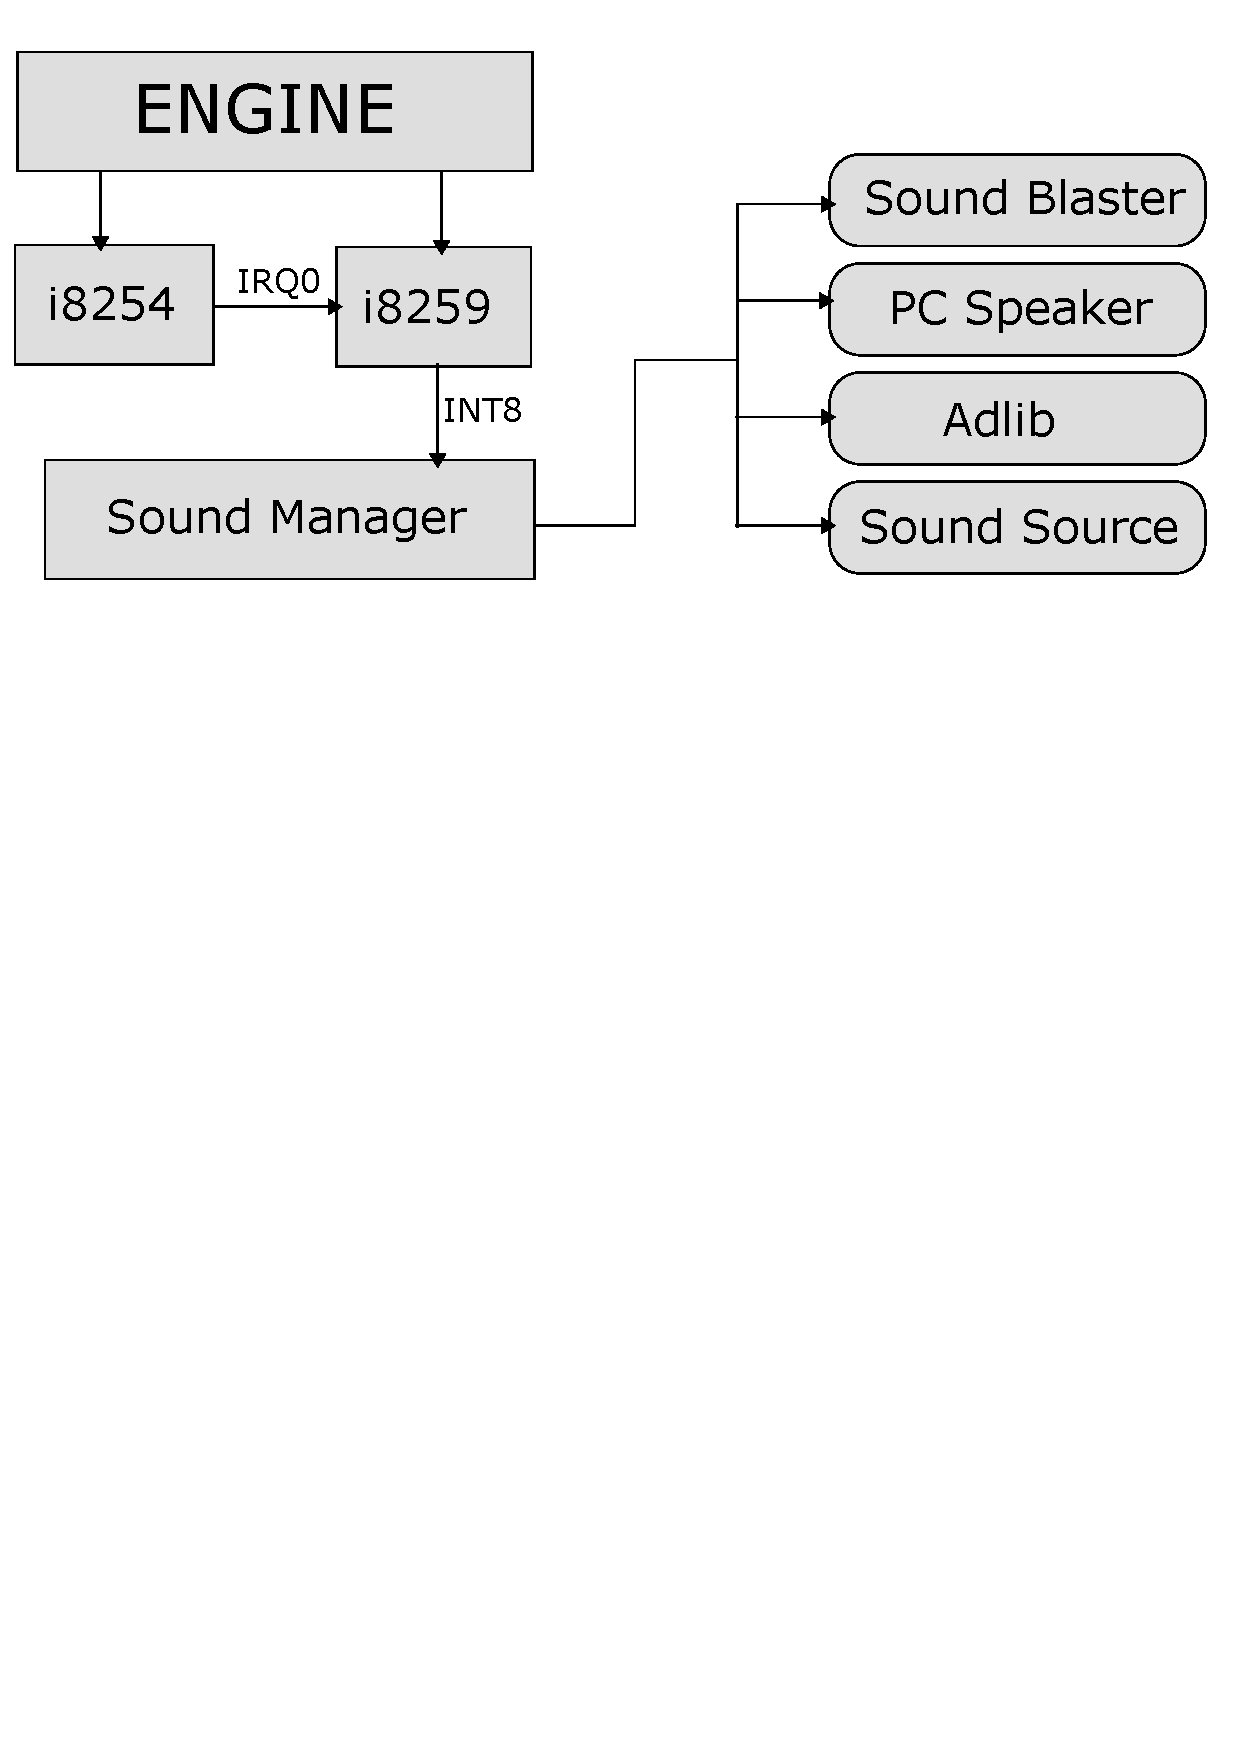
\includegraphics[width=\textwidth]{imgs/drawings/sound_manager_architecture.pdf}
 \caption{Sound system architecture.}
 \end{figure}
 \par
The sound manager is described extensively in the "Sound and Music" section.

















\subsection{Input Manager (IN)}
The Input manager abstracts interactions with joystick, keyboard, and mouse. It features the boring boilerplate code to deal with PS/2, Serial, and DA-15 ports, with each using their own I/O addresses.
















\section{Startup}
As the game engine starts, it must deal with the difficulties described in Chapter \ref{chapter_hardware} \nameref{chapter_hardware}. This is where things become really interesting.





\subsection{Signon}
The first (mild) issue to deal with was the heterogeneous ecosystem of PCs on the market. With different drivers loaded and different sound cards, the engine has to figure out how much RAM is installed and whether or not it will be able to run. If not, it has to let the user know what the problem is. That was important as id Software was a small team, without the resources to help troubleshoot customer issues.\\
\par
That is what the "signon" screen is for: self diagnostics. 
\par
\begin{figure}[H]
\centering
\fullimage{signon.png}
\caption{Signon screen.}
\end{figure}
\par
Besides showing recognized devices such as mouse, joystick, and sound cards, the signon screen's most important metric is labeled "MAIN". Due to the architecture described in Chapter \ref{chapter_hardware} \nameref{chapter_hardware}, a DOS program has only 640KiB of RAM available. Each driver loaded by the user takes away from these 640KiB. If DOS cannot load the executable in RAM, the user will see the following error message:\\
\par 
\begin{minipage}{\textwidth}
\lstinputlisting[language=C]{code/OutOfMemory.txt}
\end{minipage}
\par
The signon screen shows that Wolf3D needs at least 320KiB of Conventional RAM. John Romero wrote a release note to help people understand what was going on and avoid angry calls. You can read it in the annex under "The 640KB Barrier".\\
\par 
At the time signon is displayed, the only loaded manager is the Memory Manager. There is not even a filesystem for the engine to access yet. That is why the palette and the signon screen are compiled within the executable. This is done so they are loaded in RAM by the operating system (DOS) loader. All the engine does is load the palette into the VGA, copy the signon bitmap from RAM to VRAM, and fill the "thermometer" blocks with green or yellow based on what was detected.\\
\par
\begin{minipage}{\textwidth}
\lstinputlisting[language=C]{code/signonscreen.c}
\end{minipage}
After that screen, the \cw{introscn} variable (using 320x200 bytes = 64,000 bytes) is unloaded from RAM to make more room for runtime.\\
\par




















\subsection{Solving the VGA Problem}
Chapter \ref{chapter_hardware} \nameref{chapter_hardware} left us with an unresolved issue: all the VGA modes lack double buffering capability.\\
\par
 The most appealing mode (13h) offers a single framebuffer at a resolution of 320x200 non-square pixels with 256 indexed colors. The Chain-4 chipset in the VGA circuitry automatically maps the RAM starting at \cw{A0000h} to the four VRAM banks. 
 \par
 \begin{figure}[H]
\centering
      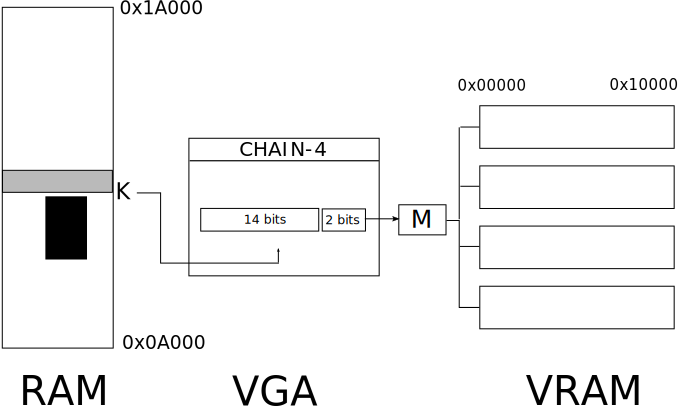
\includegraphics[width=\textwidth]{imgs/drawings/mode_13h.pdf}
      \caption{Chain-4 chipset between RAM and VRAM routes I/Os operations.}
\end{figure}

This mapping system is also called "chaining". Because 2 bits out of the address are used to route a write/read operation to a bank, only 14 bits are used for the actual offset in the bank. Since 14 bits can only address 16384 values, this system results in 75\% of VRAM left unusable.\\

\begin{figure}[H]
\centering
 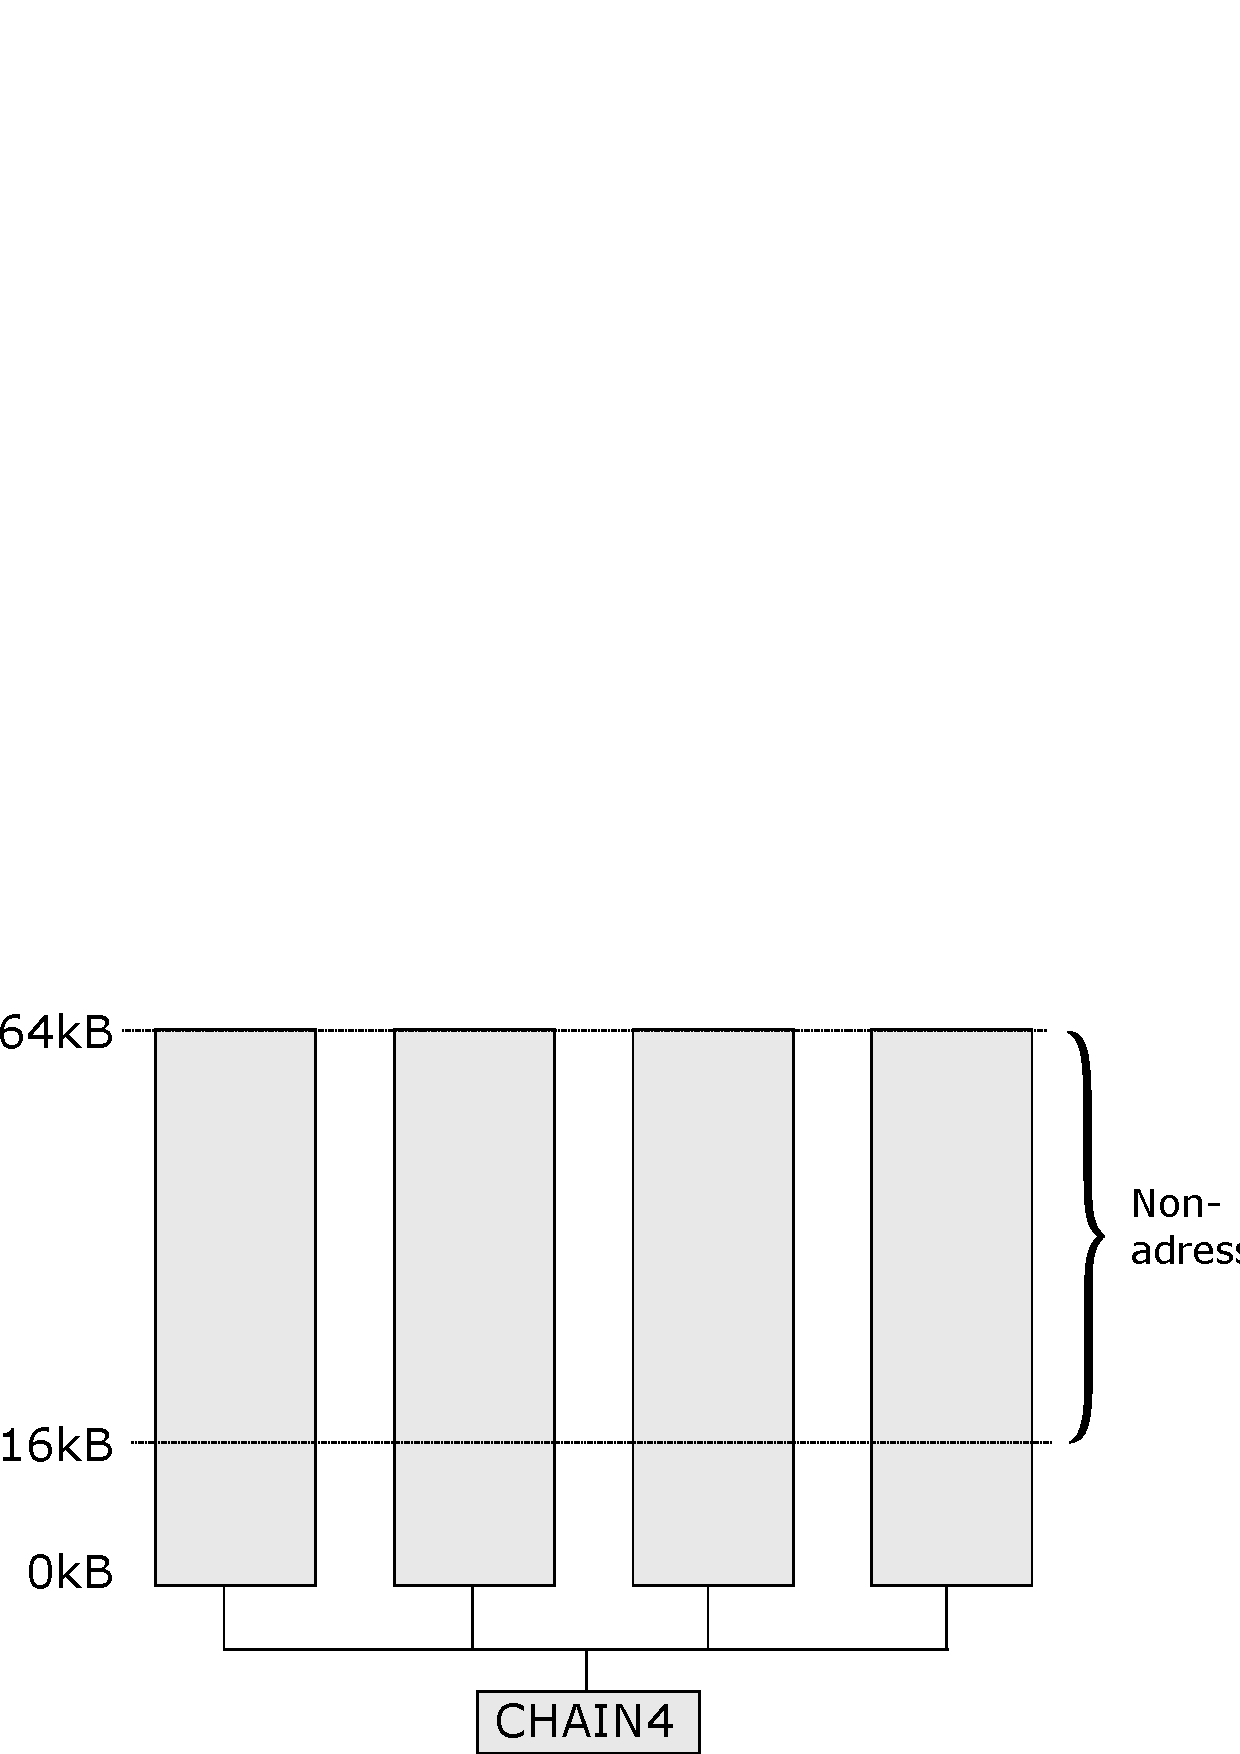
\includegraphics[width=\textwidth]{imgs/drawings/vga_layout/wasted_vga_ram.pdf}
  \caption{Chain-4 fakes one continuous VRAM bank but wastes 75\% of the VRAM.}
 \end{figure}

 \par
 The waste is really the fault of the Chain-4 chip. However it turns out it is possible to disable this. The technique was popularized by Michael Abrash in Dr. Dobb's Journal of July 1991. In his article he described what he coined Mode-X. An undocumented sequence of operations disabling Chain-4 allows for a resolution of 320x240 square pixels (since the ratio is 4:3) and full access to the 256KiB of RAM.\\
 \par
 Wolfenstein 3D does things slightly differently. It disables Chain-4 but keeps resolution at 320x200. This mode was coined Mode-Y one year later\footnote{rec.games.programmer, February 10th, 1992}. \\
 \par
 There are two reasons the team did not use 320x240 square pixels. Despite its advantage for artists, a screen using Mode-Y is 320x200 = 64,000 pixels, which represents 17\% fewer pixels compared to Mode-X with 320x240 = 76,800 pixels. The engine already struggled to reach an acceptable framerate, so Mode-X was simply too many pixels per frame. It would have also been inconvenient to artists since Deluxe Paint ran in Mode 13h which has non-square pixels. This would have created an awkward pipeline where assets would have been created and rendered at different resolutions.
 \par
 \par
  \begin{minipage}{\textwidth}
\lstinputlisting[language=C]{code/init_vga.c}
\end{minipage}
 \par

The magic happens in function \cw{VL\_DePlaneVGA} where VGA registers are manipulated to tweak what the BIOS had setup in Mode 13h. \\

 \par
 \begin{minipage}{\textwidth}
\lstinputlisting[language=C]{code/unchaining.c}
\end{minipage}

 \par
 The VGA registers of the Sequence Controller and CRT Controller are setup to divide the 256KiB VRAM into four parts.
 \begin{itemize}\label{SetupPages}
 \item 64,000 bytes for Framebuffer 0
 \item 64,000 bytes for Framebuffer 1
 \item 64,000 bytes for Framebuffer 2
 \item 70,144 bytes for Graphic assets
\end{itemize}
\par
\begin{figure}[H]
\centering
 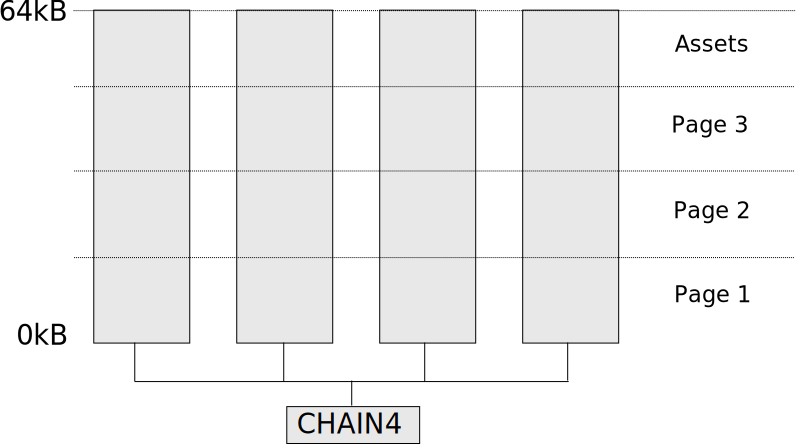
\includegraphics[width=\textwidth]{imgs/drawings/vga_layout/vga_ram_architecture.pdf}
 \end{figure}
\par
But the engine is not done yet. Tweaking Mode \cw{13h} into Mode-Y solves one big problem but introduces two smaller ones: one regarding speed and one regarding correctness.\\
\par
Let's look at speed first. With Chain-4 out of the picture the developer is now in charge of selecting the bank to write to. This can easily be done with a simple function.\\
\par
 \par
 \begin{minipage}{\textwidth}
\lstinputlisting[language=C]{code/select_plan.c}
\end{minipage}
 \par

Now the code sample from the hardware chapter on page \pageref{clearvga} to clear the screen only adds a modulo.\\
\par
\par
\begin{minipage}{\textwidth}
\lstinputlisting[language=C]{code/cleanScreenNaive.c}
\end{minipage}
\par
The code looks innocuous, but as simple as it is, it cannot run at more than a few frames per second\footnote{5 frames per seconds on a 386DX-40 with Cirrus Logic VGA card.}. The problem is we replaced something done in hardware with something done in software. The \cw{outp} instructions are simply too slow.\\
\par
The solution is to change how we draw to the screen. Instead of drawing horizontally first we need to draw vertically first in order to minimize the number of bank switches.\\
\par
\begin{minipage}{\textwidth}
\lstinputlisting[language=C]{code/cleanScreenClever.c}
\end{minipage}

\par
This code runs twice as fast\footnote{10 frames per seconds on a 386DX-40 with Cirrus Logic VGA card.} since just 200 slow \cw{outp} instructions are used\footnote{To reach 70 frames per second is possible by using fewer instructions thanks to \cw{REP STOSW} instruction.}.\\
\par
This speed consideration has a fundamental impact on the engine: to draw anything fast with the VGA, it has to be drawn vertically. Everything in the engine is drawn this way: walls, sprites, menus. The ramifications of this hardware constraint are felt all the way down to how assets are stored in RAM: rotated 90 degrees and woven to match the VGA bank layout. This is described in detail in section \ref{drawingSprites} "\nameref{drawingSprites}".\\

\par
The second issue introduced by Mode-Y is about correctness. With three pages available, the engine draws in page 1, then page 2, then page 3, and then goes back to page 1. This solves tearing and allows the engine to never block on vsync since it always has a valid framebuffer to draw to. Changing pages is done by instructing the CRT Controller that it should scan a framebuffer at a different offset after the next vsync.\\
\par
The CRT Controller scan offset is a 16 bit value which is updated with a little bit of assembly writing to a VGA register: first the high byte and then the low byte as follows.\\
\par
\begin{minipage}{\textwidth}
\lstinputlisting[language={[x86masm]Assembler}]{code/pageflip.c}
\end{minipage}
This code looks like it would work, but there is a major flaw with it. If you were to run it, every once in a while the expected screen shown below...

 \begin{figure}[H]
\centering
 \scaledimage{0.95}{full_screen.png}
 \end{figure}
...would instead appear distorted:\\
\par
 \begin{figure}[H]
\centering
 \fullimage{crtc_scanstart_problem.png}
 \end{figure}
\par
This glitch shows both misalignment and parts of two pages. This problem has to do with atomicity. The CRTC starting address is a 16 bit value but the \cw{out} instruction can only write 8 bits at a time. If the pages are setup one after another like this.
\par
\begin{figure}[H]
 \centering
 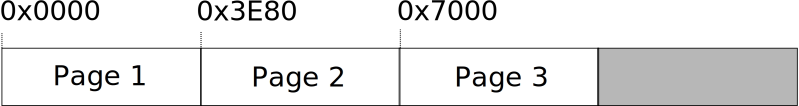
\includegraphics[width=\textwidth]{imgs/drawings/triple_pages_trick.pdf}
\end{figure}
\par
In VRAM, Page 1 is at 0x0000, page 2 at 0x3E80 and page 3 at 0x7000. Instructing the CRTC to use page 2 instead of page 1 requires updating the high byte 0x00 to 0x3E and the low byte 0x00 to 0x80. Since updates are not atomic, poor timing could result in the CRTC picking up a value of 0x3E00 instead of 0x3E80:\\
\par
\par
\begin{minipage}{\textwidth}
\lstinputlisting[language={[x86masm]Assembler}]{code/pageflip_error.c}
\end{minipage}
\par
How do you update atomically a 2 byte value with a 1 byte operation? Take a look at how Wolfenstein sets up its pages:\\
\par
\begin{minipage}{\textwidth}
\begin{flushright}
\lstinputlisting[language=C]{code/vga_setup_pages.c}
\end{flushright}
\end{minipage}
\par
Notice how it uses a value of 208 for the height of a framebuffer.  At first, this doesn't make sense as the screen is 200 pixels tall. I thought it was a typo (after all \cw{0} and \cw{8} are visually close) but this was done intentionally. The trick here is to use a little bit of padding after each page so the addresses only differ by their high byte value.


\par
\begin{figure}[H]
 \centering
 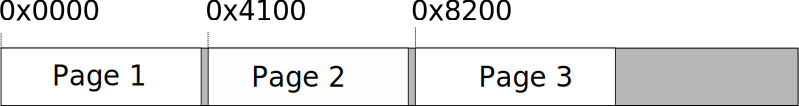
\includegraphics[width=\textwidth]{imgs/drawings/triple_pages_trick_padding.pdf}
 \caption{A little padding between pages makes all starting address a multiple of 256.}
\end{figure}
\par



\par
Now page 0 is at 0x0000, page 1 at 0x4100 and page 2 at 0x8200. Moving from any page to another requires updating only the high 8 bits, which makes flipping buffer an atomic operation.\\












\subsection{Profound Carnage}
After the signon screen comes the "rating" screen. There were no official ratings for video games in 1991 since the ESRB\footnote{Entertainment Software Rating Board, the organization in charge of assigning age and content ratings.} would not be established until 1994 in response to criticisms of excessive violence (a.k.a Doom) or sexual content. The team came up with their own self-proclaimed PC-13: the now legendary "Profound Carnage-13".\\
\begin{figure}[H]
\centering
\fullimage{pg13.png}
\caption{This program has been rated PC "Profound Carnage" - 13.}
\end{figure}







\end{document}
